%--------------------------------------
%ELECTROTECHNIQUE - SCHEMA DE LIAISON A LA TERRE
%--------------------------------------

%utiliser les environnement \begin{comment} \end{comment} pour mettre en commentaire le préambule une fois la programmation appelée dans le document maître (!ne pas oublier de mettre en commentaire \end{document}!)

\begin{comment}

\documentclass[a4paper, 11pt, twoside, fleqn]{memoir}

\usepackage{AOCDTF}

\marqueurchapitre

%lien d'édition des figures Tikz sur le site mathcha.io (rajouter le lien d'une modification effectuée sur la figure tikz avec le nom du modificateur car il n'y a qu'un lien par compte)

%lien mathcha Bruno Douchy : https://www.mathcha.io/editor/nlpozt7QSeWtkXQqWyi5zjE93SXrZeriPKxP5

%--------------------------------------
%corps du document
%--------------------------------------

\begin{document} %corps du document
	\openleft %début de chapitre à gauche

\end{comment}

\begin{figure}[H]
\caption{Piquet de terre\label{fig:piquet_terre}}


\tikzset{every picture/.style={line width=0.75pt}} %set default line width to 0.75pt        

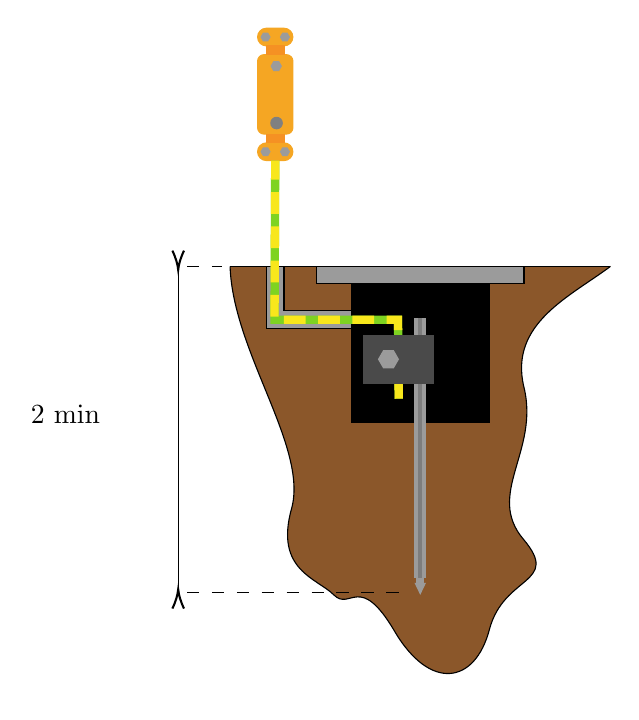
\begin{tikzpicture}[x=0.75pt,y=0.75pt,yscale=-0.85,xscale=0.85]
%uncomment if require: \path (0,484); %set diagram left start at 0, and has height of 484

%Rounded Rect [id:dp6359600964219599] 
\draw  [color={rgb, 255:red, 245; green, 166; blue, 35 }  ,draw opacity=1 ][fill={rgb, 255:red, 245; green, 166; blue, 35 }  ,fill opacity=1 ] (430,80) .. controls (430,77.24) and (432.24,75) .. (435,75) -- (445,75) .. controls (447.76,75) and (450,77.24) .. (450,80) -- (450,80) .. controls (450,82.76) and (447.76,85) .. (445,85) -- (435,85) .. controls (432.24,85) and (430,82.76) .. (430,80) -- cycle ;
%Shape: Regular Polygon [id:dp5335311391934556] 
\draw  [color={rgb, 255:red, 155; green, 155; blue, 155 }  ,draw opacity=1 ][fill={rgb, 255:red, 155; green, 155; blue, 155 }  ,fill opacity=1 ] (448,80) -- (446.75,82.17) -- (444.25,82.17) -- (443,80) -- (444.25,77.83) -- (446.75,77.83) -- cycle ;
%Shape: Regular Polygon [id:dp7077127128502503] 
\draw  [color={rgb, 255:red, 155; green, 155; blue, 155 }  ,draw opacity=1 ][fill={rgb, 255:red, 155; green, 155; blue, 155 }  ,fill opacity=1 ] (437,80) -- (435.75,82.17) -- (433.25,82.17) -- (432,80) -- (433.25,77.83) -- (435.75,77.83) -- cycle ;

%Rounded Rect [id:dp26376134008390595] 
\draw  [color={rgb, 255:red, 245; green, 166; blue, 35 }  ,draw opacity=1 ][fill={rgb, 255:red, 245; green, 166; blue, 35 }  ,fill opacity=1 ] (430,145) .. controls (430,142.24) and (432.24,140) .. (435,140) -- (445,140) .. controls (447.76,140) and (450,142.24) .. (450,145) -- (450,145) .. controls (450,147.76) and (447.76,150) .. (445,150) -- (435,150) .. controls (432.24,150) and (430,147.76) .. (430,145) -- cycle ;
%Shape: Regular Polygon [id:dp6433620371225686] 
\draw  [color={rgb, 255:red, 155; green, 155; blue, 155 }  ,draw opacity=1 ][fill={rgb, 255:red, 155; green, 155; blue, 155 }  ,fill opacity=1 ] (448,145) -- (446.75,147.17) -- (444.25,147.17) -- (443,145) -- (444.25,142.83) -- (446.75,142.83) -- cycle ;
%Shape: Regular Polygon [id:dp6874144748844591] 
\draw  [color={rgb, 255:red, 155; green, 155; blue, 155 }  ,draw opacity=1 ][fill={rgb, 255:red, 155; green, 155; blue, 155 }  ,fill opacity=1 ] (437,145) -- (435.75,147.17) -- (433.25,147.17) -- (432,145) -- (433.25,142.83) -- (435.75,142.83) -- cycle ;

%Rounded Rect [id:dp6592130378481749] 
\draw  [color={rgb, 255:red, 245; green, 166; blue, 35 }  ,draw opacity=1 ][fill={rgb, 255:red, 245; green, 166; blue, 35 }  ,fill opacity=1 ] (430,93.67) .. controls (430,91.64) and (431.64,90) .. (433.67,90) -- (446.33,90) .. controls (448.36,90) and (450,91.64) .. (450,93.67) -- (450,131.33) .. controls (450,133.36) and (448.36,135) .. (446.33,135) -- (433.67,135) .. controls (431.64,135) and (430,133.36) .. (430,131.33) -- cycle ;
%Shape: Regular Polygon [id:dp28570519258745464] 
\draw  [color={rgb, 255:red, 155; green, 155; blue, 155 }  ,draw opacity=1 ][fill={rgb, 255:red, 155; green, 155; blue, 155 }  ,fill opacity=1 ] (443.43,96.48) -- (442,98.96) -- (439.14,98.96) -- (437.7,96.48) -- (439.14,94) -- (442,94) -- cycle ;
%Shape: Rectangle [id:dp1437469136470797] 
\draw  [color={rgb, 255:red, 245; green, 145; blue, 35 }  ,draw opacity=1 ][fill={rgb, 255:red, 245; green, 145; blue, 35 }  ,fill opacity=1 ] (445,135) -- (435,135) -- (435,140) -- (445,140) -- cycle ;
%Shape: Rectangle [id:dp5260720882019565] 
\draw  [color={rgb, 255:red, 245; green, 145; blue, 35 }  ,draw opacity=1 ][fill={rgb, 255:red, 245; green, 145; blue, 35 }  ,fill opacity=1 ] (445,85) -- (435,85) -- (435,90) -- (445,90) -- cycle ;
%Shape: Circle [id:dp38824432139246823] 
\draw  [color={rgb, 255:red, 128; green, 128; blue, 128 }  ,draw opacity=1 ][fill={rgb, 255:red, 128; green, 128; blue, 128 }  ,fill opacity=1 ] (444,128.75) .. controls (444,126.96) and (442.54,125.5) .. (440.75,125.5) .. controls (438.96,125.5) and (437.5,126.96) .. (437.5,128.75) .. controls (437.5,130.54) and (438.96,132) .. (440.75,132) .. controls (442.54,132) and (444,130.54) .. (444,128.75) -- cycle ;

%Curve Lines [id:da1902694494170415] 
\draw [fill={rgb, 255:red, 139; green, 87; blue, 42 }  ,fill opacity=1 ]   (414.41,210) .. controls (416.02,258.76) and (458.92,312.57) .. (449.23,347.41) .. controls (439.53,382.24) and (463.78,386.73) .. (473.21,396.19) .. controls (482.63,405.66) and (487.64,382.87) .. (507.69,416.85) .. controls (527.73,450.84) and (553.21,446.92) .. (561.4,415.79) .. controls (569.6,384.67) and (602.15,390.07) .. (580.62,364.59) .. controls (559.09,339.12) and (589.8,314.72) .. (581,278.6) .. controls (572.2,242.47) and (607.23,227.08) .. (630,210) ;
%Shape: Rectangle [id:dp6184966297023284] 
\draw  [color={rgb, 255:red, 0; green, 0; blue, 0 }  ,draw opacity=1 ][fill={rgb, 255:red, 155; green, 155; blue, 155 }  ,fill opacity=1 ] (463.41,210) -- (581,210) -- (581,219.8) -- (463.41,219.8) -- cycle ;
%Straight Lines [id:da003175631258122258] 
\draw [fill={rgb, 255:red, 139; green, 87; blue, 42 }  ,fill opacity=1 ]   (414.41,210) -- (630,210) ;
%Shape: Rectangle [id:dp15550713014547501] 
\draw  [fill={rgb, 255:red, 0; green, 0; blue, 0 }  ,fill opacity=1 ] (483.01,219.8) -- (561.4,219.8) -- (561.4,298.2) -- (483.01,298.2) -- cycle ;
%Straight Lines [id:da6327089569131619] 
\draw [color={rgb, 255:red, 155; green, 155; blue, 155 }  ,draw opacity=1 ][line width=3]    (522.2,239.4) -- (522.2,390.19) ;
\draw [shift={(522.2,396.19)}, rotate = 270] [fill={rgb, 255:red, 155; green, 155; blue, 155 }  ,fill opacity=1 ][line width=0.08]  [draw opacity=0] (6.79,-3.26) -- (0,0) -- (6.79,3.26) -- cycle    ;
%Straight Lines [id:da7643156131849724] 
\draw [color={rgb, 255:red, 155; green, 155; blue, 155 }  ,draw opacity=1 ][line width=4.5]    (522.2,239.4) -- (522.2,386.39) ;
%Straight Lines [id:da9437529376818724] 
\draw [color={rgb, 255:red, 74; green, 74; blue, 74 }  ,draw opacity=0.37 ][line width=1.5]    (522.2,239.4) -- (522.2,386.39) ;
%Straight Lines [id:da45205830376086187] 
\draw [color={rgb, 255:red, 0; green, 0; blue, 0 }  ,draw opacity=1 ][fill={rgb, 255:red, 155; green, 155; blue, 155 }  ,fill opacity=1 ]   (435,210) -- (445,210) -- (445,235) -- (483,235) -- (483,245) -- (435,245) -- cycle ;
%Straight Lines [id:da9689359180145172] 
\draw [color={rgb, 255:red, 126; green, 211; blue, 33 }  ,draw opacity=1 ][line width=3]    (440,150) -- (439.6,240.26) -- (509.6,240.26) -- (510,285) ;
%Straight Lines [id:da44161159619032986] 
\draw [color={rgb, 255:red, 248; green, 231; blue, 28 }  ,draw opacity=1 ][line width=3]  [dash pattern={on 7.88pt off 4.5pt}]  (510,285) -- (509.6,240.26) -- (439.6,240.26) -- (440,150) ;
%Shape: Rectangle [id:dp5856416399734485] 
\draw  [color={rgb, 255:red, 74; green, 74; blue, 74 }  ,draw opacity=1 ][fill={rgb, 255:red, 74; green, 74; blue, 74 }  ,fill opacity=1 ] (490.2,249.16) -- (529.4,249.16) -- (529.4,276.11) -- (490.2,276.11) -- cycle ;
%Shape: Regular Polygon [id:dp7503784010969258] 
\draw  [color={rgb, 255:red, 155; green, 155; blue, 155 }  ,draw opacity=1 ][fill={rgb, 255:red, 155; green, 155; blue, 155 }  ,fill opacity=1 ] (509.8,262.63) -- (506.99,267.49) -- (501.38,267.49) -- (498.57,262.63) -- (501.38,257.77) -- (506.99,257.77) -- cycle ;
%Straight Lines [id:da7038410601404053] 
\draw    (385,212) -- (385,393) ;
\draw [shift={(385,393)}, rotate = 90] [color={rgb, 255:red, 0; green, 0; blue, 0 }  ][line width=0.75]    (10.93,-3.29) .. controls (6.95,-1.4) and (3.31,-0.3) .. (0,0) .. controls (3.31,0.3) and (6.95,1.4) .. (10.93,3.29)   ;
\draw [shift={(385,212)}, rotate = 270] [color={rgb, 255:red, 0; green, 0; blue, 0 }  ][line width=0.75]    (10.93,-3.29) .. controls (6.95,-1.4) and (3.31,-0.3) .. (0,0) .. controls (3.31,0.3) and (6.95,1.4) .. (10.93,3.29)   ;
%Straight Lines [id:da2144228436087714] 
\draw  [dash pattern={on 4.5pt off 4.5pt}]  (390,210) -- (410,210) ;
%Straight Lines [id:da5349045349345829] 
\draw  [dash pattern={on 4.5pt off 4.5pt}]  (390,395) -- (515,395) ;

% Text Node
\draw (300,287) node [anchor=north west][inner sep=0.75pt]   [align=left] {\SI{2}{\meter} min};


\end{tikzpicture}



\end{figure}

%\end{document}

